%% LyX 2.0.6 created this file.  For more info, see http://www.lyx.org/.
%% Do not edit unless you really know what you are doing.
\documentclass{article}
\usepackage[latin9]{inputenc}
\usepackage{amsmath}
\usepackage{amssymb}
\usepackage{graphicx}

\makeatletter
%%%%%%%%%%%%%%%%%%%%%%%%%%%%%% User specified LaTeX commands.
%% This document created by Scientific Word (R) Version 3.0


\usepackage{pstcol}\usepackage{pstricks}\usepackage{egameps}\usepackage{amsfonts}%TCIDATA{OutputFilter=latex2.dll}
%TCIDATA{CSTFile=LaTeX article (bright).cst}
%TCIDATA{Created=Thu Oct 07 14:29:47 2004}
%TCIDATA{LastRevised=Fri Oct 15 22:19:39 2004}
%TCIDATA{<META NAME="GraphicsSave" CONTENT="32">}
%TCIDATA{<META NAME="DocumentShell" CONTENT="General\Blank Document">}
%TCIDATA{Language=American English}
\newtheorem{theorem}{Theorem}
\newtheorem{acknowledgement}[theorem]{Acknowledgement}
\newtheorem{algorithm}[theorem]{Algorithm}
\newtheorem{assumption}[theorem]{Assumption}
\newtheorem{axiom}[theorem]{Axiom}
\newtheorem{case}[theorem]{Case}
\newtheorem{claim}[theorem]{Claim}
\newtheorem{conclusion}[theorem]{Conclusion}
\newtheorem{condition}[theorem]{Condition}
\newtheorem{conjecture}[theorem]{Conjecture}
\newtheorem{corollary}[theorem]{Corollary}
\newtheorem{criterion}[theorem]{Criterion}
\newtheorem{definition}[theorem]{Definition}
\newtheorem{example}[theorem]{Example}
\newtheorem{exercise}[theorem]{Exercise}
\newtheorem{lemma}[theorem]{Lemma}
\newtheorem{notation}[theorem]{Notation}
\newtheorem{problem}[theorem]{Problem}
\newtheorem{proposition}[theorem]{Proposition}
\newtheorem{remark}[theorem]{Remark}
\newtheorem{solution}[theorem]{Solution}
\newtheorem{summary}[theorem]{Summary}
\newenvironment{proof}[1][Proof]{\textbf{#1.} }{\ \rule{0.5em}{0.5em}}



\makeatother

\begin{document}

\title{Uncertainty}


\author{Michael Peters}


\date{\today}

\maketitle
 


\section{Lotteries}

In many problems in economics, people are forced to make decisions
without knowing exactly what the consequences will be. For example,
when you buy a lottery ticket, you don't know whether or not you will
win when you buy the ticket. There are many important problems like
this. If you buy car insurance, you hope you won't need it, but you
aren't sure. A politician who spends time and money running for public
office is not sure whether or not they will be elected. A drug company
that invests in developing a new drug is not sure whether or not it
will actually work. A corporate insider who sells shares using inside
information is never sure whether or not they will be caught.

One way to think about such problems is to use the concept of a \emph{lottery}.
A lottery is a pair of objects. The first, $\mathcal{X}$, is a list
of possible consequences of a decision. The second is a list $p=\left\{ p_{1},p_{2},\dots p_{n}\right\} $
of probabilities with which you think that each of the consequences
will occur. The number of probabilities you list, $n$, is exactly
equal to the number of consequences in $\mathcal{X}$. For example,
if you buy a lottery ticket, the set of consequences consists of two
things, you either win or lose. Each of these consequences occurs
with probability $\frac{1}{2}$. If you sell stock based on an insider's
tip, you either get away with it, or you don't. More generally, there
could be many consequences. If you open a new restaurant you might
sell 1 or 2 or 3, or any number of meals per week. The set of consequences
could be very large.

In this definition, the set of consequences could be very general.
In particular, each of the consequences could be a lottery. A lottery
over lotteries is called a \emph{compound lottery}. Lotteries over
anything else are called \emph{simple} lotteries. As an abstract example,
consider the following game. I will flip a coin and if the coin comes
up heads right away, I will give you \$2. If it comes up tails, I
will flip the coin again. If it comes up heads on the second flip,
I will pay you \$4. If it comes up tails, we stop and you get nothing.
This is a simple example of a compound lottery. The first of the two
lotteries has a single consequence, you receive \$2 (of course you
get this consequence with probability 1). The second lottery has two
possibly consequences - either you get \$4 or you get nothing. In
this second lottery, each consequence occurs with equal probability.
The compound lottery involves $\frac{1}{2}$ chance that you will
play the first lottery and get \$2 for sure. Then there is $\frac{1}{2}$
chance that you will play the second lottery and get either \$4 or
\$0.

It should be clear to you that this compound lottery is pretty much
the same thing as a simple lottery where the consequences are that
you receive either \$2, \$4 or \$0 with probabilities $\frac{1}{2}$,
$\frac{1}{4}$, and $\frac{1}{4}$. This type of lottery is sometimes
referred to as the \emph{reduced} lottery associated with the original
compound lottery.


\subsection{Monty Hall}

We normally assume that compound lotteries and the reduced lotteries
associated with them can be used interchangeably. This isn't always
as straightforward as in the example above. In the following problem,
it is very easy to make a mistake calculating the reduced lottery.
You are a contestant in a game show, and are given the choice of three
doors. Behind one door is \$1 million which you will win if you happen
to open this door. There is nothing behind the other doors, and if
you pick one of them you will win nothing. Once you choose one of
the doors, the host will open one of the remaining doors and show
you that it contains no prize. You are then given the option to change
from the door you picked in the first place, to the remaining door.
The problem is to decide whether or not to switch doors.

This is a compound lottery in which the prize is first placed randomly
behind a door, then after observing where the prize is, the host randomly
opens one of the remaining doors. It appears that the prize is equally
likely to be behind either of the three doors, so it can't matter
whether you switch or not after the host opens the door. However,
you will do better on average in this game if you always switch doors.
You might be able to see this from the following casual reasoning
- the prize could be behind any of the three doors. If it is behind
the door that you chose, then it would, of course, be a mistake to
switch. In either of the other alternatives, switching doors will
win you the prize. To put it another way, the host will actually tell
you which door contains the prize in two of the three situations you
might face. Following his advice won't always work, but it will most
of the time.

Another way to think through the problem is to try to compute the
reduced lottery that you actually face when you hold on to your original
choice, and the one you face when you switch. The first part of the
lottery involves the placement of the prize. With probability $\frac{1}{3}$
it is placed behind either of the three doors.\ The second part of
the lottery is the host's announcement about the door that doesn't
contain the prize. We might as well assume that you pick door $A$,
since the thing works the same way no matter which door you pick.
The lottery you get when you stick with your original choice is depicted
in Figure 1.

\begin{figure}[tbh]
\hspace*{\fill} \begin{egame}(600,380)
%
% put the initial branch at (300,240), with (x,y) direction
% (2,1), and horizontal length 200
\putbranch(300,340)(1,1){200}
%
% give the branch two actions, label it for player 1,
% and label the actions $L$ and $R$
\iiib{Door A,B or C}{$\frac{1}{3}$}{$\frac{1}{3}$}{$\frac{1}{3}$}
%
\putbranch(300,140)(1,1){75}
\ib{}{$1$}[$B,Lose$]
\putbranch(500,140)(1,1){75}
\ib{}{$1$}[$C,Lose$]
\putbranch(100,140)(1,1){75}
\iib{}{$\frac{1}{2}$}{$\frac{1}{2}$}[$B,Win$][$C,Win$]
\end{egame}
 \hspace*{\fill}\caption{You stick with your initial choice}


\label{f:one}
\end{figure}


The important part to understanding the correct strategy in this game
is to observe that the outcome of the second lottery depends both
on the outcome of the first lottery (the door where the prize is placed)
and on your choice. In Figure 1, the first set of branches shows the
various locations where the prize can be placed. The second set of
branches shows the doors that the host can open. Notice that if your
choice is $A$ and the prize is actually there, then the host can
choose completely randomly to open either door $B$ or $C$. On the
other hand, if the prize is behind doors $B$ or $C$, then the host
doesn't have any choice and is forced to open a door that effectively
reveals the location of the prize.

Figure 2 shows what the lottery looks like in the case where you switch
doors.

\begin{figure}[tbh]
\hspace*{\fill} \begin{egame}(600,380)
%
% put the initial branch at (300,240), with (x,y) direction
% (2,1), and horizontal length 200
\putbranch(300,340)(1,1){200}
%
% give the branch two actions, label it for player 1,
% and label the actions $L$ and $R$
\iiib{Door A,B or C}{$\frac{1}{3}$}{$\frac{1}{3}$}{$\frac{1}{3}$}
%
\putbranch(300,140)(1,1){75}
\ib{}{$1$}[$B,Win$]
\putbranch(500,140)(1,1){75}
\ib{}{$1$}[$C,Win$]
\putbranch(100,140)(1,1){75}
\iib{}{$\frac{1}{2}$}{$\frac{1}{2}$}[$B,Lose$][$C,Lose$]
\end{egame}
 \hspace*{\fill}\caption{You switch choices after the host opens a door}


\label{f:otwo}
\end{figure}


Then just glancing at the outcomes in these two figures, it should
be clear that you will win two thirds of the time if you switch, but
only one third of the time if you stick with your initial choice.


\subsection{\bigskip{}
St. Petersburg}

Here is a famous reduced lottery involving coins that actually provides
most of the motivation for the approach that we currently use in economics.
This resembles the previous coin flipping problem. As before, if the
coin comes up heads on the first flip, I give you \$2, and if it comes
up tails on the first flip, I flip again. If it comes up heads on
the second flip I give you \$4, otherwise I flip again. If it comes
up heads on the third flip, I pay you \$8, otherwise I flip again.\ We
keep going until I flip a head, then if it takes me $k$ flips to
get the head, I pay you $\$2^{k}$. The set of consequences in this
reduced lottery is the set
\[
\left\{ 1,2,3,\dots,k,\dots\right\} .
\]
It won't take you too much thinking to see that the probabilities
are
\[
\left\{ \frac{1}{2},\frac{1}{4},\dots,\frac{1}{2^{k}},\dots\right\} 
\]


I am going to ask you how much you would be willing to pay me to play
this game. You could refuse to play - then you would get nothing for
sure. Or you could offer to pay me \$2 or more (you can't lose from
this choice unless you pay more than \$2). Both choices would involve
different lotteries, though one of them (not playing) is sort of degenerate.

You might try to decide whether or not to play this game by figuring
out how much you would win on average from the game. This calculation
is straightforward.\ With probability $\frac{1}{2}$ you win \$2
right away, with probability $\frac{1}{4}$ you win \$4, with probability$\dots$
$\frac{1}{2^{k}}$ you win \$2$^{k}$. Averaging all these gives
\[
\sum_{i=1}^{\infty}\frac{1}{2^{i}}2^{i}=\sum_{i=1}^{\infty}1=\infty
\]
You will never find anyone who is willing to pay an infinite amount
of money to play this game.


\section{\bigskip{}
Choosing among lotteries}

In each of the problems above, you need to choose among lotteries.
There is no obvious way to do this. However, as you actually make
the choice, I am probably safe in thinking that you will be able to
express a preference over any pair of lotteries, and that the preferences
you express will be transitive (in other words, if you say that you
prefer lottery $\left(\mathcal{X},p\right)$ to lottery $\left(\mathcal{X}^{\prime},p^{\prime}\right)$,
and you say you like lottery $\left(\mathcal{X}^{\prime},p^{\prime}\right)$
more than lottery $\left(\mathcal{X}^{\prime\prime},p^{\prime\prime}\right)$,
then I should be sure that you will prefer lottery $\left(\mathcal{X},p\right)$
to lottery $\left(\mathcal{X}^{\prime\prime},p^{\prime\prime}\right)$.

Now, if there is some set of lotteries $\mathcal{L}$ from which a
choice is to be made, I\ can ask for pairwise comparisons between
all the lotteries and eventually learn all of your preferences. To
make the notation a little simpler, let me suppose that every lottery
in my set of alternatives $\mathcal{L}$ has the same set $\mathcal{X}$
of consequences. Then I can think of a lottery as a simple list of
probabilities with which these various outcomes occur. The outcomes
don't have to be amounts of money, they can be anything imaginable,
including lotteries as you have seen. Yet, as with all choice problems
I am probably not too far off the mark by assuming you can express
a preference between \emph{every} pair of lotteries in $\mathcal{L}$,
and that the preferences you express will be transitive (which means
that if $p\succeq p^{\prime}$, and $p^{\prime}\succeq p^{\prime\prime}$
then it must be that $p\succeq p^{\prime\prime}$). If your preferences
are also continuous in an appropriate way, I will be able to represent
with a utility function $u$ in the sense that $p\succeq p^{\prime}$
if and only if $u\left(p\right)\geq u\left(p^{\prime}\right)$.

One of the more important discoveries in economics is that if your
preferences satisfy a third condition, referred to as the \emph{independence
axiom}%
\footnote{This is a bit of a misnomer. It isn't really an axiom, since it is
far from self evident.\ It is more like an assumption.%
}, then this utility function will, in fact, be linear in probabilities.
The independence axiom say this: suppose that for any three lotteries
$p$, $p^{\prime}$, and $p^{\prime\prime}$, $p\succeq p^{\prime}$
implies that for any $\lambda\in\left[0,1\right]$ 
\[
\lambda p+\left(1-\lambda\right)p^{\prime\prime}\succeq
\]
\[
\lambda p^{\prime}+\left(1-\lambda\right)p^{\prime\prime}.
\]
These last two objects are compound lotteries in which you are given
lottery $\left(\mathcal{X},p\right)$ (or $\left(\mathcal{X},p^{\prime}\right)$)
with probability $\lambda$ and lottery $\left(\mathcal{X},p^{\prime\prime}\right)$
with probability $\left(1-\lambda\right)$. If you can rank two lotteries,
you will rank them the same way if they are mixed with a common third
lottery.

For the utility function to be linear in probabilities, it means that
we will be able to find numbers $u_{i}$, one for each of the $n$
outcomes in the set $\mathcal{X}$ such that
\[
u\left(\mathcal{X},p\right)=\sum_{i=1}^{n}u_{i}p_{i}
\]
Since there is one number $u_{i}$ for each of the $n$ outcomes in
$\mathcal{X}$, it is convenient to think of $u_{i}$ as the utility
value associated with outcome $x_{i}$. If the outcomes happened to
be expressed in dollars, then we could think of the utility numbers
as representing some underlying utility for wealth. The point to be
emphasized is that the existence of the utility for wealth function
is not an assumption, but an implication of a certain method of ranking
lotteries.

This is such an important idea that it is worthwhile to see how it
works. To see it, suppose that there is a $b\in\mathcal{L}$ (the
best lottery) such that $b\succeq p$ for all $p\in\mathcal{L}$;
a $w\in\mathcal{L}$ (the worst lottery) such that $p\succeq w$ for
all $p\in\mathcal{L}$. We can now try to mimic the proof of the existence
of a utility function that we did previously. Recall that we used
monotonicity of preferences and continuity. So we will say preferences
are monotonic if $\lambda b+\left(1-\lambda\right)w\succ\lambda^{\prime}b+\left(1-\lambda^{\prime}\right)w$
if and only if $\lambda>\lambda^{\prime}$.%
\footnote{The statement $p\succ p^{\prime}$ means that $p\succeq p^{\prime}$
but not $p^{\prime}\succeq p$. The notation $p\sim p^{\prime}$ means
that $p\succeq p^{\prime}$ and $p^{\prime}\succeq p$.%
} We will say that preferences are continuous if the sets $\left\{ \lambda\in\left[0,1\right]:\lambda b+\left(1-\lambda w\right)\succeq p\right\} $
and $\left\{ \lambda\in\left[0,1\right]:p\succeq\lambda b+\left(1-\lambda\right)w\right\} $
are both closed intervals.

Now we can state the result.

\begin{theorem} If preferences are complete, transitive, continuous,
monotonic and satisfy the independence axiom, then there is a utility
function $u$ representing preferences over lotteries in $\mathcal{L}$
that is linear in probabilities. \end{theorem}

\begin{proof} The proof is constructive. Let's start by creating
the utility function. This is a function that assigns a real number
to each lottery $p\in\mathcal{L}$. To do so set
\begin{equation}
u\left(p\right)=\left\{ \lambda\in\left[0,1\right]:\lambda b+\left(1-\lambda\right)w\sim p\right\} \label{define}
\end{equation}
Notice that the $\lambda$ that satisfies this relation (warning -
it is not an equation) always exists and is unique. To see why, observe
that by completeness $\lambda^{\prime}b+\left(1-\lambda^{\prime}\right)w\succeq p$
or the reverse for every $\lambda^{\prime}\in\left[0,1\right]$. Then
\[
\left\{ \lambda\in\left[0,1\right]:\lambda b+\left(1-\lambda\right)w\succeq p\right\} \cup
\]
\[
\left\{ \lambda\in\left[0,1\right]:p\succeq\lambda b+\left(1-\lambda\right)w\right\} 
\]
is all of the interval $\left[0,1\right]$. Since both these sets
are closed by the continuity of preferences, they must have at least
one point in common. Since preferences are monotonic they can't have
more than one point in common (Prove this by contradiction.)

Next, we should show that the function $u\left(\cdot\right)$ as constructed
above, actually represents preferences $\succeq$.\ This relies on
the monotonicity of preferences and is left as an exercise.

Finally, we come to the important step - showing that the utility
function defined in (\ref{define}) above is linear in probabilities,
i.e., that 
\[
u\left(\lambda p+\left(1-\lambda\right)p^{\prime}\right)=\lambda u\left(p\right)+\left(1-\lambda\right)u\left(p^{\prime}\right)
\]
for all $\lambda$, $p$, and $p^{\prime}$. I will not write down
a series of relations - make sure that you don't mistake them for
equations. First observe that
\[
\lambda p+\left(1-\lambda\right)p^{\prime}\sim
\]
\[
\lambda\left[u\left(p\right)b+\left(1-u\left(p\right)\right)w\right]+\left(1-\lambda\right)p^{\prime}
\]
This follows from the definition of the utility function $u\left(p\right)$
and the independence axiom (in the sense that we are mixing the lotteries
$p$ and $u\left(p\right)b+\left(1-u\left(p\right)\right)w$ together
with the common third lottery $p^{\prime}$). Do the same thing again
to get
\[
\lambda\left[u\left(p\right)b+\left(1-u\left(p\right)\right)w\right]+\left(1-\lambda\right)p^{\prime}\sim
\]
\[
\lambda\left[u\left(p\right)b+\left(1-u\left(p\right)\right)w\right]+\left(1-\lambda\right)\left[u\left(p^{\prime}\right)b+\left(1-u\left(p^{\prime}\right)\right)w\right]
\]
This is a fairly complicated compound lottery (first you mix lotteries
$b$ and $w$ together using $u\left(p\right)$ and $u\left(p^{\prime}\right)$.
Then you mix the result using $\lambda$.) The reduced lottery associated
with this is
\[
\left[\lambda u\left(p\right)+\left(1-\lambda\right)u\left(p^{\prime}\right)\right]b+\left[1-\lambda u\left(p\right)-\left(1-\lambda\right)u\left(p^{\prime}\right)\right]w
\]
which, if you recall where we started, is then indifferent to $\lambda p+\left(1-\lambda\right)p^{\prime}$.
If you glance back at (\ref{define}), you will see that we have just
discovered 
\[
u\left(\lambda p+\left(1-\lambda\right)p^{\prime}\right)=\lambda u\left(p\right)+\left(1-\lambda\right)u\left(p^{\prime}\right)
\]
which is the linearity property we wanted. \end{proof}

Modern economic theory is concerned largely with problems where there
is some kind of risk or uncertainty about outcomes. In finance, this
uncertainty arises from the inherent unpredictability of asset returns.
In mechanism design (the theory of auctions and institutions), uncertainty
arises because of the inability to know the tastes of others. In game
theory, uncertainty arises because of the inability to predict exactly
how another player will behave. Expected utility is the cornerstone
of the modern approach to uncertainty, so it is probably one of the
most useful ideas that you will encounter.

It has been challenged in a number of ways. The challenges reflect
both the strength of the theory and its weakness. The strength of
the theory lies in the fact that is lays out so precisely what can
and cannot happen if the theory is true. The 'can happen' part is
good, because theories are supposed to explain things we see. The
'can't happen' part is also important since it shows what kinds of
behavior would allow us to reject the theory.

You might wonder why we need a theorem like the one above connecting
expected utility which is a model of the utility function, to the
independence axiom, which you might think of as a restriction on the
way people behave. Why couldn't we just write down a specific utility
function then somehow test that, instead of worrying about behavioral
properties like the independence axiom.

There are two reasons. The first is, that provided you buy completeness,
transitivity and continuity, the independence axiom and expected utility
are equivalent. So the independence axiom provides all the behavioral
restrictions that come from assuming the utility function is linear
in probabilities. Assumptions about utility functions will typically
make it easy to derive some restrictions on behavior, but not all
of them. Knowing all of the implications makes it far easier to construct
an effective empirical test.

The second reason is that it is quite possible to impose assumptions
on utility that have no implications at all for behavior. A trivial
example might involve assumptions about the utility value associated
with the best or worst lotteries. In any case, theorems like the one
above lay out very clearly what the additional implications of linearity
are, and how they differ from the implications of other assumptions.


\section{Empirical tests}

I'll provide an example of a challenge to expected utility that involves
experimental tests (we already described how econometric tests could
be used to test the implications of completeness and transitivity).
To describe the test, let me simplify things a bit and suppose that
the set of consequences consists of exactly three things - i.e., $\mathcal{X=}\left\{ x_{1},x_{2},x_{3}\right\} $.
The set of lotteries, $\mathcal{L}$, is then just the set of triples
of probabilities $q=\left\{ q_{1},q_{2},q_{3}\right\} $. Since the
probabilities have to sum to one, it is possible to depict $\mathcal{L}$
in a simple two dimensional diagram as in Figure \ref{lotteries}%TCIMACRO{\FRAME{ftbpFU}{3.243in}{2.5953in}{0pt}{\Qcb{The set of lotteries}%
%}{\Qlb{lotteries}}{undergrad_uncertainty_fig_lottery.eps}%
%{\special{ language "Scientific Word";  type "GRAPHIC";
%maintain-aspect-ratio TRUE;  display "USEDEF";  valid_file "F";
%width 3.243in;  height 2.5953in;  depth 0pt;  original-width 3.1981in;
%original-height 2.5538in;  cropleft "0";  croptop "1";  cropright "1";
%cropbottom "0";
%filename 'undergrad_uncertainty_fig_lottery.eps';file-properties "XNPEU";}}}%
%BeginExpansion
\begin{figure}[ptb]
\begin{centering}
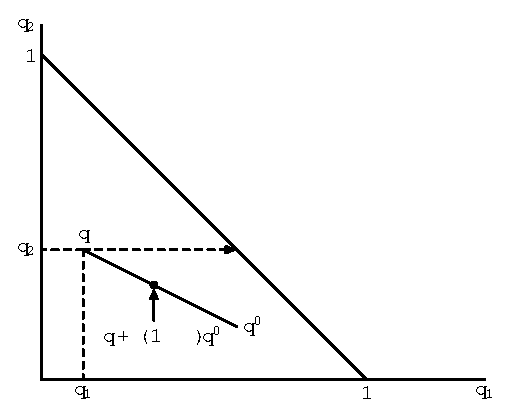
\includegraphics[width=3.243in,height=2.5953in]{undergrad_uncertainty_fig_lottery}\caption{The set of lotteries}

\par\end{centering}

\centering{}\label{lotteries}
\end{figure}


%EndExpansion


Every point in the triangle with sides of length $1$ in the diagram
above is a lottery in $\mathcal{L}$. To see this, take a point like
$q$. The coordinate on the horizontal axis, $q_{1}$ represents the
probability with which consequence $x_{1}$ occurs. The coordinate
on the vertical axis $q_{2}$ represents the probability with which
consequence $x_{2}$ occurs under lottery $q$. The probability of
consequence $x_{3}$ is just the remainder $1-q_{1}-q_{2}$. This
is given by the length of the horizontal line segment from $q$ over
to the hypotenuse of the triangle (the dashed line with the arrow
at the end in the picture). Now the lottery $q^{\prime}$ can be easily
compared to $q$. $q^{\prime}$ lies down, and to the right of $q$,
and is closer to the hypotenuse of the triangle. So, it assigns lower
probability to $x_{1}$, higher probability to $x_{2}$, and lower
probability to $x_{3}$.

Each point in the triangle represents a different simple lottery in
$\mathcal{L}$. Compound lotteries are lotteries over lotteries. For
example, one might form a lottery with two consequences - consequence
1 is the lottery $q$ while consequence $2$ is the lottery $q^{\prime}$.
Let $\lambda$ be the probability with which the first lottery $q$
is played. Then the reduced lottery associated with this compound
lottery is $\lambda q+\left(1-\lambda\right)q^{\prime}$. This lottery
is just the simple lottery that lies $\lambda/\left(1-\lambda\right)$
of the way along the line segment between $q$ and $q^{\prime}$.
This point is illustrated in Figure \ref{lotteries}.

Preferences over lotteries can then be represented by a family of
indifference curves that look exactly like the ones you are used to
using to think about preferences over commodity bundles. An indifference
curve through the lottery $q$ is set of lotteries $\tilde{q}$ that
have the same utility value as $q$. Formally, an indifference curve
is the set
\[
\left\{ \tilde{q}\in\mathcal{L}:u\left(\tilde{q}\right)=u\left(q\right)\right\} 
\]
If we use the linearity property of preferences given in our theorem
above, then the equation that defines this indifference curve is
\[
q_{1}u_{1}+q_{2}u_{2}+q_{3}u_{3}=u\left(q\right)
\]
Since $q_{3}=1-q_{1}-q_{2}$, this becomes 
\[
q_{1}u_{1}+q_{2}u_{2}+\left(1-q_{1}-q_{2}\right)u_{3}=u\left(q\right)
\]
or
\[
q_{2}=\frac{u\left(q\right)-qu_{1}-\left(1-q\right)u_{3}}{u_{2}-u_{3}}
\]
This is a linear function of $q_{1}$, which means that indifference
curves are straight lines.

To see the argument another way, go back to the independence axiom,
which states that for \emph{any }three lotteries $q$, $q^{\prime}$
and $q^{\prime\prime}$ and any $\lambda$, the lotteries $\lambda q+\left(1-\lambda\right)q^{\prime\prime}$
and $\lambda q^{\prime}+\left(1-\lambda\right)q^{\prime\prime}$ must
be ranked the same way as $q$ and $q^{\prime}$. Since this must
be true for \emph{any} three lotteries, then it must be that we can
use $q^{\prime}$ in place of $q^{\prime\prime}$ in the argument
above to conclude that $\lambda q+\left(1-\lambda\right)q^{\prime}$
and $\lambda q^{\prime}+\left(1-\lambda\right)q^{\prime}$ must be
ranked the same way as $q$ and $q^{\prime}$. Then reducing the compound
lottery, if $q\symbol{126}q^{\prime}$ then $\lambda q+\left(1-\lambda\right)q^{\prime}\symbol{126}q^{\prime}\symbol{126}q$.
Which means that every lottery on the line segment between $q$ and
$q^{\prime}$ must be indifferent to $q$. That is just another way
of saying that the indifference curves are straight lines.

It is a bit hard to deal with indifference. If you offer me $q$ and
$q^{\prime}$ in an experiment I will choose one of the them. I might
strictly prefer the one I\ pick, or I might be indifferent between
them. It would be hard to figure this out in practice. Fortunately,
the independence axiom provides a much stronger condition that gets
around this. You can see this condition in Figure \ref{parallel}.
%TCIMACRO{\FRAME{ftbpFU}{3.243in}{2.5953in}{0pt}{\Qcb{Parallel Indifference
%Curves}}{\Qlb{parallel}}{undergrad_uncertainty_fig_parallel.eps}%
%{\special{ language "Scientific Word";  type "GRAPHIC";
%maintain-aspect-ratio TRUE;  display "USEDEF";  valid_file "F";
%width 3.243in;  height 2.5953in;  depth 0pt;  original-width 3.1981in;
%original-height 2.5538in;  cropleft "0";  croptop "1";  cropright "1";
%cropbottom "0";
%filename 'undergrad_uncertainty_fig_parallel.eps';file-properties "XNPEU";}}}%
%BeginExpansion
\begin{figure}[ptb]
\begin{centering}
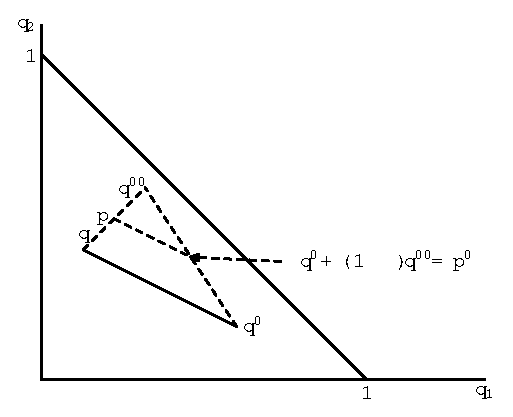
\includegraphics[width=3.243in,height=2.5953in]{undergrad_uncertainty_fig_parallel}\caption{Parallel Indifference Curves}

\par\end{centering}

\centering{}\label{parallel}
\end{figure}


%EndExpansion
In the Figure, $q$ and $q^{\prime}$ are two lotteries on the same
indifference curve. By the previous argument the indifference curve
connecting them is a straight line. Choose some other lottery like
$p$ which strictly preferred to $q$. We shall try to determine what
the indifference curve looks like through the lottery $p$.

Draw a line segment from $q$ through $p$ to some third lottery $q^{\prime\prime}$
as in the figure. Suppose that $\lambda$ is such that $p=\lambda q+\left(1-\lambda\right)q^{\prime}$.
Now since $q$ $\sim q^{\prime}$, we have by the independence axiom
that
\[
p=\lambda q+\left(1-\lambda\right)q^{\prime\prime}\sim\lambda q^{\prime}+\left(1-\lambda q^{\prime\prime}\right)
\]
Now the line segment from $p$ to $\lambda q^{\prime}+\left(1-\lambda q^{\prime\prime}\right)$
is evidently parallel to the line segment from $q$ to $q^{\prime}$,
so the indifference curve through $p$ must be parallel to the indifference
curve through $q$. In other words, all the indifference curves are
parallel to one another when the independence axiom holds.

Now this is something that can be tested with an experiment. Simply
present an experimental subject a choice between two lotteries and
observe their choice. Once you see what their choice is, present them
another two lotteries whose probabilities are scaled in such a way
that knowing that the indifference curves are all straight and parallel
to one another will allow you to predict their choice in the second
lottery.

This is the experiment that was suggested by Allais. The consequences
are monetary with $x_{1}=\$100$, $x_{2}=\$50$ and $x_{3}=0$. The
first pair of lotteries offered to the experimental subject are
\[
q=\left\{ 0,1,0\right\} 
\]
and 
\[
q^{\prime}=\left\{ .1,.89,.01\right\} 
\]
In other words, you can have either a sure \$50, or take a chance
on getting \$100 with a small chance that you will lose everything.
Most people are inclined to take the sure \$50 in this case.

The second pair of lotteries is
\[
p=\left\{ 0,.11,.89\right\} 
\]
and 
\[
p^{\prime}=\left\{ .1,0,.9\right\} 
\]
In this case, you probably won't win anything with either lottery.
Lottery $p$ offers you a small chance to earn \$50. Lottery $p^{\prime}$
gives you a slightly smaller chance of earning $\$100$, but also
increases the probability with which you won't win anything. Most
people are inclined to take the chance in this case and opt for lottery
$p^{\prime}$ - perhaps because they are so unlikely to win anything
they feel there is nothing to lose in going for the \$100.

You should plot each of these four lotteries in a Figure like the
one above. You will see that the line segment joining $q$ and $q^{\prime}$
is parallel to the line segment joining $p$ and $p^{\prime}$. If
indifference curves are all straight lines, parallel to one another,
anyone who chooses $q$ over $q^{\prime}$ must also choose $p$ over
$p^{\prime}$ (just draw in the indifference curve that would induce
them to choose $q$ over $q^{\prime}$ then shift it down to see what
they will do with $p$ and $p^{\prime})$.
\end{document}
